% Plantilla para un Trabajo Fin de Grado de la Universidad de Granada,
% adaptada para el Doble Grado en Ingeniería Informática y Matemáticas.
%
%  Autor: Mario Román.
%  Licencia: GNU GPLv2.
%
% Esta plantilla es una adaptación al castellano de la plantilla
% classicthesis de André Miede, que puede obtenerse en:
%  https://ctan.org/tex-archive/macros/latex/contrib/classicthesis?lang=en
% La plantilla original se licencia en GNU GPLv2.
%
% Esta plantilla usa símbolos de la Universidad de Granada sujetos a la normativa
% de identidad visual corporativa, que puede encontrarse en:
% http://secretariageneral.ugr.es/pages/ivc/normativa
%
% La compilación se realiza con las siguientes instrucciones:
%   pdflatex --shell-escape main.tex
%   bibtex main
%   pdflatex --shell-escape main.tex
%   pdflatex --shell-escape main.tex

% Opciones del tipo de documento
\documentclass[twoside,openright,titlepage,numbers=noenddot,headinclude,footinclude=true,
cleardoublepage=empty,abstractoff,BCOR=5mm,paper=a4,fontsize=12pt,main=spanish,pdfstartpage=1]{scrreprt}

% Paquetes de latex que se cargan al inicio. Cubren la entrada de
% texto, gráficos, código fuente y símbolos.
\PassOptionsToPackage{table,dvipsnames}{xcolor}

\usepackage[utf8]{inputenc}
\usepackage[T1]{fontenc}
\usepackage{fixltx2e}
\usepackage{graphicx} % Inclusión de imágenes.
\usepackage{grffile}  % Distintos formatos para imágenes.
\usepackage{longtable} % Tablas multipágina.
\usepackage{wrapfig} % Coloca texto alrededor de una figura.
\usepackage{rotating}
\usepackage[normalem]{ulem}
\usepackage{amsmath}
\usepackage{dsfont}
\usepackage{textcomp}
\usepackage{amssymb}
\usepackage{capt-of}
\usepackage[colorlinks=true]{hyperref}
\usepackage{tikz} % Diagramas conmutativos.
\usepackage{minted} % Código fuente.
\usepackage[numbers]{natbib}
\usepackage{booktabs} % Para tablas de figuras (ejemplo en salesman)
\usepackage{listings} % Código
\usepackage{comment}
\usepackage{float}
\usepackage[table]{xcolor}
\PassOptionsToPackage{table,dvipsnames}{xcolor}

\lstset{
	basicstyle=\ttfamily,%
	breaklines=true,%
	captionpos=b,                    % sets the caption-position to bottom
  tabsize=2,	                   % sets default tabsize to 2 spaces
  frame=none,
  numbers=left,
  xleftmargin=18pt,
  stepnumber=1,
  aboveskip=12pt,
  showstringspaces=false,
  keywordstyle=\bfseries,
  commentstyle=\itshape,
  numberstyle=\scriptsize\bfseries,
  %morekeywords={sage},
}


% Operadores

\DeclareMathOperator{\gr}{gr}
\DeclareMathOperator{\mcd}{mcd}

\lstset{ frame=Ltb,
framerule=0pt,
aboveskip=0.5cm,
framextopmargin=3pt,
framexbottommargin=3pt,
framexleftmargin=0.4cm,
framesep=0pt,
rulesep=.4pt,
backgroundcolor=\color{white},
rulesepcolor=\color{black},
%
stringstyle=\ttfamily,
showstringspaces = false,
basicstyle=\small\ttfamily,
commentstyle=\color{gray},
keywordstyle=\bfseries,
%
numbers=left,
numbersep=15pt,
numberstyle=\tiny,
numberfirstline = false,
breaklines=true,
}


\definecolor{codegreen}{rgb}{0,0.6,0}
\definecolor{codegray}{rgb}{0.5,0.5,0.5}
\definecolor{codepurple}{rgb}{0.58,0,0.82}
\definecolor{backcolour}{rgb}{0.95,0.95,0.92}


\lstdefinestyle{mystyle}{
  language=C++,
    commentstyle=\color{codegreen},
    keywordstyle=\color{magenta},
    numberstyle=\tiny\color{codegray},
    stringstyle=\color{codepurple},
    basicstyle=\ttfamily\footnotesize,
}

\lstset{style=mystyle}
% Plantilla classicthesis
\usepackage[beramono,eulerchapternumbers,linedheaders,parts,a5paper,dottedtoc,
manychapters,pdfspacing]{classicthesis}

% Geometría y espaciado de párrafos.
\setcounter{secnumdepth}{0}
\usepackage{enumitem}
\setitemize{noitemsep,topsep=0pt,parsep=0pt,partopsep=0pt}
\setlist[enumerate]{topsep=0pt,itemsep=-1ex,partopsep=1ex,parsep=1ex}
\usepackage[top=1in, bottom=1.5in, left=1in, right=1in]{geometry}
\setlength\itemsep{0em}
\setlength{\parindent}{0pt}
\usepackage{parskip}
\usepackage{setspace}
\usepackage{amsmath}


% Profundidad de la tabla de contenidos.
\setcounter{secnumdepth}{3}

% Usa el paquete minted para mostrar trozos de código.
% Pueden seleccionarse el lenguaje apropiado y el estilo del código.
\usepackage{minted}
\usemintedstyle{colorful}
\setminted{fontsize=\small}
\setminted[haskell]{linenos=false,fontsize=\small}
\renewcommand{\theFancyVerbLine}{\sffamily\textcolor[rgb]{0.5,0.5,1.0}{\oldstylenums{\arabic{FancyVerbLine}}}}

% Path para las imágenes
\graphicspath{{figures/}}

% Archivos de configuración.
%------------------------
% Bibliotecas para matemáticas de latex
%------------------------
\usepackage{amsthm}
\usepackage{amsmath}
\usepackage{tikz}
\usepackage{tikz-cd}
\usetikzlibrary{shapes,fit}
\usepackage{bussproofs}
\EnableBpAbbreviations{}
\usepackage{mathtools}
\usepackage{scalerel}
\usepackage{stmaryrd}


%------------------------
% Estilos para los teoremas
%------------------------
\theoremstyle{plain}
\newtheorem{theorem}{Teorema}
\newtheorem{proposition}{Proposición}
\newtheorem{lemma}{Lema}
\newtheorem{corollary}{Corolario}

\theoremstyle{definition}
\newtheorem{definition}{Definición}

% Change the proof style so it's in English and add \qed at the end.
\renewenvironment{proof}{{\bfseries Demostración.}}{\qed}

\theoremstyle{remark}
\newtheorem{remark}{Observación}
\newtheorem{exampleth}{Ejemplo}

% New style for postulates so they are tabulated
\makeatletter
\newtheoremstyle{indented}
	{3pt}% space before
	{3pt}% space after
	{\addtolength{\@totalleftmargin}{3.5em}
		\addtolength{\linewidth}{-3.5em}
		\parshape 1 3.5em \linewidth}% body font
	{}% indent
	{\bfseries}% header font
	{.}% punctuation
	{.5em}% after theorem header
	{}% header specification (empty for default)
\makeatother

% Apply the new style
\theoremstyle{indented}
\newtheorem{postulate}{Postulate}
\newtheorem*{postulate 3'}{Postulate 3'}
\newtheorem*{postulate 2'}{Projective Measurement}

%------------------------
% Macros
% ------------------------

\newcommand*{\B}{\mathbb{B}}
\newcommand*{\C}{\mathds{C}}
\newcommand*{\R}{\mathbb{R}}
\newcommand*{\ra}{\rangle}
\newcommand*{\la}{\langle}

% Para poner sonrisa sobre puntos suspensivos. Uso: \overplace{n}{\dotsc}
\newcommand{\overplace}[2]{%
	\overset{\substack{#1\\\smile}}{#2}%
}

% Para añadir un salto de línea al nuevo párrafo. Use: \newparagraph
\newcommand{\newparagraph}[1]{\paragraph{#1}\mbox{}\\}  % En macros.tex se almacenan las opciones y comandos para escribir matemáticas.
% ****************************************************************************************************
% classicthesis-config.tex 
% formerly known as loadpackages.sty, classicthesis-ldpkg.sty, and classicthesis-preamble.sty 
% Use it at the beginning of your ClassicThesis.tex, or as a LaTeX Preamble 
% in your ClassicThesis.{tex,lyx} with \input{classicthesis-config}
% ****************************************************************************************************  
% If you like the classicthesis, then I would appreciate a postcard. 
% My address can be found in the file ClassicThesis.pdf. A collection 
% of the postcards I received so far is available online at 
% http://postcards.miede.de
% ****************************************************************************************************


% ****************************************************************************************************
% 0. Set the encoding of your files. UTF-8 is the only sensible encoding nowadays. If you can't read
% äöüßáéçèê∂åëæƒÏ€ then change the encoding setting in your editor, not the line below. If your editor
% does not support utf8 use another editor!
% ****************************************************************************************************
\PassOptionsToPackage{utf8x}{inputenc}
	\usepackage{inputenc}

% ****************************************************************************************************
% 1. Configure classicthesis for your needs here, e.g., remove "drafting" below 
% in order to deactivate the time-stamp on the pages
% ****************************************************************************************************
\PassOptionsToPackage{eulerchapternumbers,listings,drafting,%
		pdfspacing,%floatperchapter,%linedheaders,%
                subfig,beramono,eulermath,parts,dottedtoc}{classicthesis}                                        
% ********************************************************************
% Available options for classicthesis.sty 
% (see ClassicThesis.pdf for more information):
% drafting
% parts nochapters linedheaders
% eulerchapternumbers beramono eulermath pdfspacing minionprospacing
% tocaligned dottedtoc manychapters
% listings floatperchapter subfig
% ********************************************************************

% ****************************************************************************************************
% 2. Personal data and user ad-hoc commands
% ****************************************************************************************************
\newcommand{\myTitle}{Prácticas DDSI\xspace}
\newcommand{\mySubtitle}{An Homage to The Elements of Typographic Style\xspace}
\newcommand{\myDegree}{Doktor-Ingenieur (Dr.-Ing.)\xspace}
\newcommand{\myName}{André Miede\xspace}
\newcommand{\myProf}{Put name here\xspace}
\newcommand{\myOtherProf}{Put name here\xspace}
\newcommand{\mySupervisor}{Put name here\xspace}
\newcommand{\myFaculty}{Put data here\xspace}
\newcommand{\myDepartment}{Put data here\xspace}
\newcommand{\myUni}{Put data here\xspace}
\newcommand{\myLocation}{Saarbrücken\xspace}
\newcommand{\myTime}{September 2015\xspace}
%\newcommand{\myVersion}{version 4.2\xspace}

% ********************************************************************
% Setup, finetuning, and useful commands
% ********************************************************************
\newcounter{dummy} % necessary for correct hyperlinks (to index, bib, etc.)
\newlength{\abcd} % for ab..z string length calculation
\providecommand{\mLyX}{L\kern-.1667em\lower.25em\hbox{Y}\kern-.125emX\@}
\newcommand{\ie}{i.\,e.}
\newcommand{\Ie}{I.\,e.}
\newcommand{\eg}{e.\,g.}
\newcommand{\Eg}{E.\,g.} 
% ****************************************************************************************************


% ****************************************************************************************************
% 3. Loading some handy packages
% ****************************************************************************************************
% ******************************************************************** 
% Packages with options that might require adjustments
% ******************************************************************** 
%\PassOptionsToPackage{ngerman,american}{babel}   % change this to your language(s)
% Spanish languages need extra options in order to work with this template
% \PassOptionsToPackage{es-lcroman,spanish}{babel}
\usepackage[main=spanish]{babel}


%\usepackage{csquotes}
% \PassOptionsToPackage{%
%     %backend=biber, %instead of bibtex
% 	backend=bibtex8,bibencoding=ascii,%
% 	language=auto,%
% 	style=alpha,%
%     %style=authoryear-comp, % Author 1999, 2010
%     %bibstyle=authoryear,dashed=false, % dashed: substitute rep. author with ---
%     sorting=nyt, % name, year, title
%     maxbibnames=10, % default: 3, et al.
%     %backref=true,%
%     natbib=true % natbib compatibility mode (\citep and \citet still work)
% }{biblatex}
%     \usepackage{biblatex}

% \PassOptionsToPackage{fleqn}{amsmath}       % math environments and more by the AMS 
%     \usepackage{amsmath}

% ******************************************************************** 
% General useful packages
% ******************************************************************** 
\PassOptionsToPackage{T1}{fontenc} % T2A for cyrillics
    \usepackage{fontenc}     
\usepackage{textcomp} % fix warning with missing font shapes
\usepackage{scrhack} % fix warnings when using KOMA with listings package          
\usepackage{xspace} % to get the spacing after macros right  
\usepackage{mparhack} % get marginpar right
\usepackage{fixltx2e} % fixes some LaTeX stuff --> since 2015 in the LaTeX kernel (see below)
%\usepackage[latest]{latexrelease} % will be used once available in more distributions (ISSUE #107)
\PassOptionsToPackage{printonlyused,smaller}{acronym} 
    \usepackage{acronym} % nice macros for handling all acronyms in the thesis
    %\renewcommand{\bflabel}[1]{{#1}\hfill} % fix the list of acronyms --> no longer working
    %\renewcommand*{\acsfont}[1]{\textsc{#1}} 
    \renewcommand*{\aclabelfont}[1]{\acsfont{#1}}
% ****************************************************************************************************


% ****************************************************************************************************
% 4. Setup floats: tables, (sub)figures, and captions
% ****************************************************************************************************
\usepackage{tabularx} % better tables
    \setlength{\extrarowheight}{3pt} % increase table row height
\newcommand{\tableheadline}[1]{\multicolumn{1}{c}{\spacedlowsmallcaps{#1}}}
\newcommand{\myfloatalign}{\centering} % to be used with each float for alignment
\usepackage{caption}
% Thanks to cgnieder and Claus Lahiri
% http://tex.stackexchange.com/questions/69349/spacedlowsmallcaps-in-caption-label
% [REMOVED DUE TO OTHER PROBLEMS, SEE ISSUE #82]    
%\DeclareCaptionLabelFormat{smallcaps}{\bothIfFirst{#1}{~}\MakeTextLowercase{\textsc{#2}}}
%\captionsetup{font=small,labelformat=smallcaps} % format=hang,
\captionsetup{font=small} % format=hang,
\usepackage{subfig}  
% ****************************************************************************************************


% ****************************************************************************************************
% 5. Setup code listings
% ****************************************************************************************************
% \usepackage{listings} 
% %\lstset{emph={trueIndex,root},emphstyle=\color{BlueViolet}}%\underbar} % for special keywords
% \lstset{language={Haskell},morekeywords={PassOptionsToPackage,selectlanguage},keywordstyle=\color{RoyalBlue},basicstyle=\small\ttfamily,commentstyle=\color{Green}\ttfamily,stringstyle=\rmfamily,numbers=none,numberstyle=\scriptsize,stepnumber=5,numbersep=8pt,showstringspaces=false,breaklines=true,belowcaptionskip=.75\baselineskip} 
% ****************************************************************************************************             


% ****************************************************************************************************
% 6. PDFLaTeX, hyperreferences and citation backreferences
% ****************************************************************************************************
% ********************************************************************
% Using PDFLaTeX
% ********************************************************************
\PassOptionsToPackage{pdftex,hyperfootnotes=false,pdfpagelabels}{hyperref}
    \usepackage{hyperref}  % backref linktocpage pagebackref
\pdfcompresslevel=9
\pdfadjustspacing=1 
\PassOptionsToPackage{pdftex}{graphicx}
    \usepackage{graphicx} 
 

% ********************************************************************
% Hyperreferences
% ********************************************************************
\hypersetup{%
    %draft, % = no hyperlinking at all (useful in b/w printouts)
    colorlinks=true, linktocpage=true, pdfstartpage=3, pdfstartview=FitV,%
    % uncomment the following line if you want to have black links (e.g., for printing)
    %colorlinks=false, linktocpage=false, pdfstartpage=3, pdfstartview=FitV, pdfborder={0 0 0},%
    breaklinks=true, pdfpagemode=UseNone, pageanchor=true, pdfpagemode=UseOutlines,%
    plainpages=false, bookmarksnumbered, bookmarksopen=true, bookmarksopenlevel=1,%
    hypertexnames=true, pdfhighlight=/O,%nesting=true,%frenchlinks,%
    urlcolor=webbrown, linkcolor=RoyalBlue, citecolor=webgreen, %pagecolor=RoyalBlue,%
    %urlcolor=Black, linkcolor=Black, citecolor=Black, %pagecolor=Black,%
    pdftitle={\myTitle},%
    pdfauthor={\textcopyright\ \myName, \myUni, \myFaculty},%
    pdfsubject={},%
    pdfkeywords={},%
    pdfcreator={pdfLaTeX},%
    pdfproducer={LaTeX with hyperref and classicthesis}%
}   

% ********************************************************************
% Setup autoreferences
% ********************************************************************
% There are some issues regarding autorefnames
% http://www.ureader.de/msg/136221647.aspx
% http://www.tex.ac.uk/cgi-bin/texfaq2html?label=latexwords
% you have to redefine the makros for the 
% language you use, e.g., american, ngerman
% (as chosen when loading babel/AtBeginDocument)
% ********************************************************************
\makeatletter
\@ifpackageloaded{babel}%
    {%
        
       \addto\extrasamerican{%
			\renewcommand*{\figureautorefname}{Figure}%
			\renewcommand*{\tableautorefname}{Table}%
			\renewcommand*{\partautorefname}{Part}%
			\renewcommand*{\chapterautorefname}{Chapter}%
			\renewcommand*{\sectionautorefname}{Section}%
			\renewcommand*{\subsectionautorefname}{Section}%
			\renewcommand*{\subsubsectionautorefname}{Section}%     
                }%
       \addto\extrasngerman{% 
			\renewcommand*{\paragraphautorefname}{Absatz}%
			\renewcommand*{\subparagraphautorefname}{Unterabsatz}%
			\renewcommand*{\footnoteautorefname}{Fu\"snote}%
			\renewcommand*{\FancyVerbLineautorefname}{Zeile}%
			\renewcommand*{\theoremautorefname}{Theorem}%
			\renewcommand*{\appendixautorefname}{Anhang}%
			\renewcommand*{\equationautorefname}{Gleichung}%        
			\renewcommand*{\itemautorefname}{Punkt}%
                }%  
            % Fix to getting autorefs for subfigures right (thanks to Belinda Vogt for changing the definition)
            \providecommand{\subfigureautorefname}{\figureautorefname}%             
    }{\relax}
\makeatother


% ****************************************************************************************************
% 7. Last calls before the bar closes
% ****************************************************************************************************
% ********************************************************************
% Development Stuff
% ********************************************************************
\listfiles
%\PassOptionsToPackage{l2tabu,orthodox,abort}{nag}
%   \usepackage{nag}
%\PassOptionsToPackage{warning, all}{onlyamsmath}
%   \usepackage{onlyamsmath}

% ********************************************************************
% Last, but not least...
% ********************************************************************
\usepackage{classicthesis} 
% ****************************************************************************************************


% ****************************************************************************************************
% 8. Further adjustments (experimental)
% ****************************************************************************************************
% ********************************************************************
% Changing the text area
% ********************************************************************
%\linespread{1.05} % a bit more for Palatino
%\areaset[current]{312pt}{761pt} % 686 (factor 2.2) + 33 head + 42 head \the\footskip
%\setlength{\marginparwidth}{7em}%
%\setlength{\marginparsep}{2em}%

% ********************************************************************
% Using different fonts
% ********************************************************************
%\usepackage[oldstylenums]{kpfonts} % oldstyle notextcomp
%\usepackage[osf]{libertine}
%\usepackage[light,condensed,math]{iwona}
%\renewcommand{\sfdefault}{iwona}
%\usepackage{lmodern} % <-- no osf support :-(
%\usepackage{cfr-lm} % 
%\usepackage[urw-garamond]{mathdesign} <-- no osf support :-(
%\usepackage[default,osfigures]{opensans} % scale=0.95 
%\usepackage[sfdefault]{FiraSans}
% **************************************************************************************************** % En classicthesis-config.tex se almacenan las opciones propias de la plantilla.

% Color institucional UGR
% \definecolor{ugrColor}{HTML}{ed1c3e} % Versión clara.
\definecolor{ugrColor}{HTML}{FFA500}  % Usado en el título.
\definecolor{ugrColor2}{HTML}{FFA500} % Usado en las secciones.
% Prácticas DDSI
% Definición de colores
\definecolor{rojo}{RGB}{200,0,0}
\definecolor{azul}{RGB}{0,70,160}
\definecolor{verde}{RGB}{0,160,70}

% Datos de portada
\usepackage{titling} % Facilita los datos de la portada
\author{Ismael Sallami Moreno \\ Jesús Rodríguez González \\ Fernando José Gracia Choin \\ Sergio Calvo González \\ Javier Niño Sánchez} 
\title{Otros modelos de datos para SI}

% Portada
\usepackage{datetime}
\renewcommand\maketitle{
  \begin{titlepage}
    \begin{addmargin}[-0cm]{-0cm}
      \begin{center}
        \normalsize  
        \hfill
        \vfill
        \vspace{1.8cm}

        \spacedallcaps{Diseño y Desarrollo de Sistemas de Información: Trabajo Tema 4} \\ \medskip 
        \small{\spacedallcaps{Doble grado en Ingeniería Informática + ADE}} \\  \bigskip\bigskip
        \vspace{1.5cm}

        \begingroup
        \LARGE{\color{ugrColor}\spacedallcaps{\textbf{\thetitle}}} \\ \bigskip
        \endgroup

        \vfill
        \vspace{1.5cm}

        \textbf{Autores}\\
        \spacedlowsmallcaps{\theauthor}

        \hfill
        \vspace{1.7cm}

        \quad
        
\includegraphics{figures/etsiit_logo.png}

        \spacedlowsmallcaps{E.T.S. de Ingenierías Informática y de Telecomunicación} \\ \medskip
        \vspace{1.0cm}
        %\textit{Curso académico 2021-2022}
        \textit{Granada, a \today}

        \vfill                      

      \end{center}  
    \end{addmargin}       
  \end{titlepage}}
\usepackage{wallpaper}
\usepackage[main=spanish]{babel}


\usepackage{slantsc}

% Algoritmos

\usepackage[linesnumbered, onelanguage, ruled]{algorithm2e}
\SetAlCapFnt{\sffamily}
\SetAlCapNameFnt{\sffamily}
\newcommand\mycommentfont[1]{\sffamily\textcolor{darkgray}{#1}}
\SetCommentSty{mycommentfont}
%\SetAlFnt{\sffamily}
%\SetKwSty{sffamily}
\SetAlCapSkip{.5em}
\SetAlgoCaptionLayout{raggedright}
\SetAlgorithmName{Algoritmo}{Algoritmo}{Lista de algoritmos}
%\SetAlgoSkip{medskip}
\SetAlgoInsideSkip{medskip}

% Entorno algoritmo con líneas pero caption debajo
\makeatletter
\newenvironment{Ualgorithm}[1][htpb]{\def\@algocf@post@ruled{\color{gray}\hrule  height\algoheightrule\kern6pt\relax}%
\def\@algocf@capt@ruled{under}%
\setlength\algotitleheightrule{0pt}%
\SetAlgoCaptionLayout{raggedright}%
\begin{algorithm}[#1]}
{\end{algorithm}}
\makeatother

% Comandos
\theoremstyle{plain}
\newtheorem{problemth}{Problema}

%Tikz styles para la práctica 2 de ddsi
\usepackage{tikz}
\usetikzlibrary{
    calc,           % Para cálculos de coordenadas
    positioning,    % Para colocar nodos de manera relativa (ej: below of)
    shapes,         % Para formas avanzadas (diamantes, elipses, etc.)
    arrows,         % Para estilos de flechas
    fit             % Para ajustar un nodo a un conjunto de nodos
}

\tikzstyle{agente} = [
    rectangle, draw, thick, 
    minimum width=2.5cm, minimum height=1cm, 
    fill=blue!15, text centered, 
    font=\bfseries\small
] % Agente Externo

\tikzstyle{proceso} = [
    rectangle, rounded corners=5pt, draw, thick, 
    minimum width=2.5cm, minimum height=1cm, 
    fill=green!20, text centered, 
    font=\bfseries\small
] % Proceso

\tikzset{
    almacen/.style={
        rectangle,
        minimum width=3cm,
        minimum height=1cm,
        fill=yellow!20,
        text centered,
        inner sep=5pt,
        font=\bfseries\small,
        draw=none, % no dibuja borde automático
        append after command={
            \pgfextra{
                % Dibuja todos los lados excepto el derecho
                \draw[thick]
                    (\tikzlastnode.north west) --
                    (\tikzlastnode.north east) --
                    (\tikzlastnode.south east) --
                    (\tikzlastnode.south west) -- cycle;
                % Borra (no dibujamos) el lado derecho
                \draw[white, line width=3pt]
                    (\tikzlastnode.north east) --
                    (\tikzlastnode.south east);
            }
        }
    }
}

\tikzset{
  hexnode/.style={
      draw,
      shape=regular polygon,
      regular polygon sides=6,
      minimum size=3cm,
      inner sep=10pt,
  },
  smallbox/.style={
      draw,
      rectangle,
      minimum size=1cm,
      fill=gray!20
  }
}

\tikzstyle{flujo} = [
  ->, very thick, >=stealth, 
  font=\small
] % Flujo de datos

\tikzset{
  flujo/.style={->, thick, shorten >=6pt, shorten <=6pt, to path={-| (\tikztotarget)}}
}

\tikzset{
  flujo/.style={
    ->, thick,
    shorten >=6pt, shorten <=6pt,
    rounded corners=8pt, % esquinas redondeadas para rodear nodos
  },
  autoavoid/.style={
    to path={
      % Intenta evitar otras flechas usando out/in y bend
      [rounded corners=12pt]
      |- (\tikztotarget)
      \tikztonodes
    }
  }
}

\tikzstyle{iflujo} = [
  <-, very thick, >=stealth, 
  font=\small
] % Flujo de datos inverso

\tikzset{
  iflujo/.style={<-, thick, shorten >=6pt, shorten <=6pt, to path={-| (\tikztotarget)}}
}

\tikzset{
  iflujo/.style={
    <-, thick,
    shorten >=6pt, shorten <=6pt,
    rounded corners=8pt, % esquinas redondeadas para rodear nodos
  },
  autoavoid/.style={
    to path={
      % Intenta evitar otras flechas usando out/in y bend
      [rounded corners=12pt]
      |- (\tikztotarget)
      \tikztonodes
    }
  }
}

\makeatletter
\@addtoreset{chapter}{part}
\makeatother




\begin{document}


\ThisULCornerWallPaper{1}{figures/ugrA4_orange.pdf}
\maketitle


\onehalfspacing

% Indice
\tableofcontents
\newpage



% \chapter{Ejemplo}
% \input{chapters/ejemplo_requisito.tex}

% ----------------------------------------------------
% CAPÍTULOS DE LOS INTEGRANTES DEL GRUPO
% ----------------------------------------------------
% Cada alumno edita SOLAMENTE su archivo en la carpeta chapters/

\chapter{Modelo Objeto-Relacional (Ismael)}
\label{ch:ismael}

En este capítulo se implementa el subsistema de \textbf{Publicidad} del sistema EKIS utilizando el modelo Objeto-Relacional de Oracle Database. Este enfoque permite tratar los anuncios no como registros planos, sino como objetos complejos que encapsulan tanto sus datos (título, fechas) como su lógica de negocio (verificación de vigencia) y estructuras anidadas (lista de características del público objetivo).

\section{Instalación y Configuración del Entorno}

Para la realización de esta práctica, se ha optado por desplegar Oracle Database 21c Express Edition (XE) utilizando tecnología de contenedores Docker sobre un sistema operativo Ubuntu Linux. Esta arquitectura permite aislar el SGBD del sistema anfitrión, evitando conflictos de dependencias y facilitando una instalación limpia.

El proceso técnico seguido fue el siguiente:

\begin{enumerate}
    \item \textbf{Despliegue del contenedor:} Se utilizó la imagen \texttt{gvenzl/oracle-xe}, mapeando el puerto 1521 para permitir conexiones externas.
    \item \textbf{Conexión mediante SQL*Plus:} Se accedió a la interfaz de línea de comandos del contenedor para realizar las tareas administrativas.
    \item \textbf{Creación de usuario:} Se creó un usuario específico para la práctica (\texttt{c\#\#ismael}) siguiendo la nomenclatura de usuarios comunes de la arquitectura \textit{multitenant} de Oracle (prefijo \texttt{c\#\#}), otorgándole permisos de conexión y recursos ilimitados.
\end{enumerate}

La siguiente figura muestra la secuencia de comandos utilizada en la terminal para verificar la instalación, conectar al sistema y preparar el usuario de trabajo:

\begin{figure}[H]
    \centering
    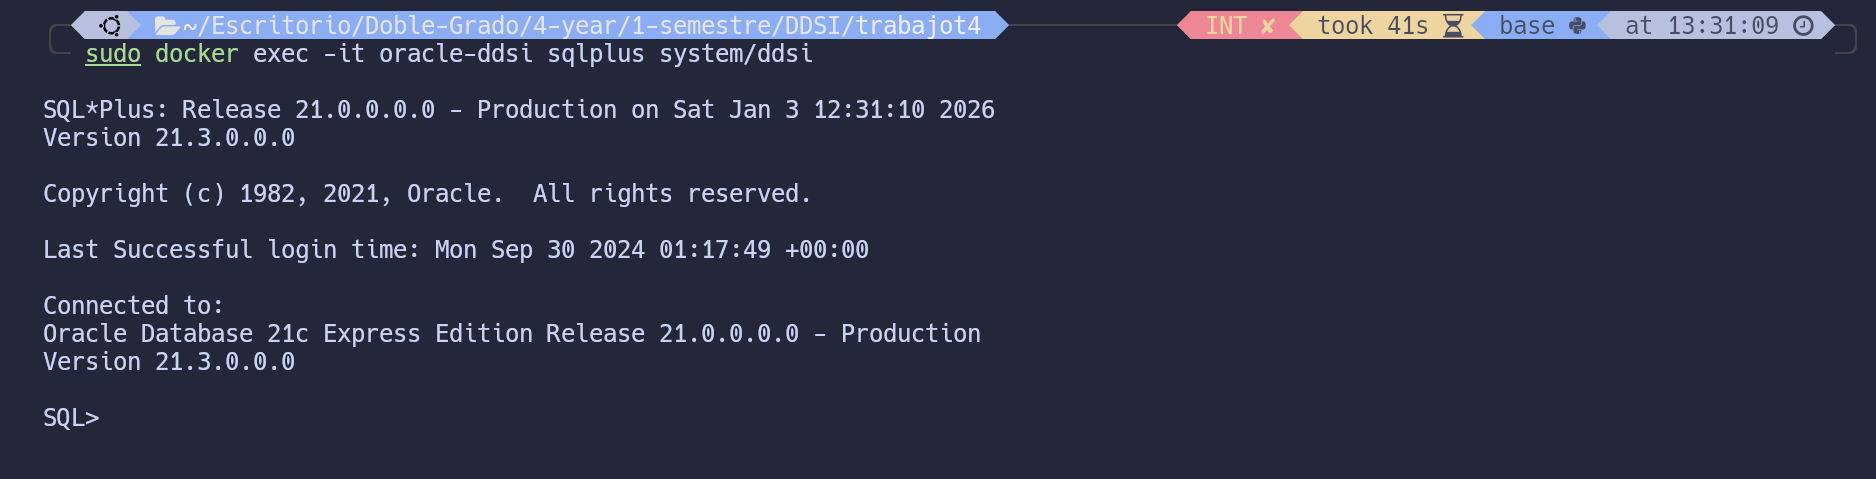
\includegraphics[width=1.0\textwidth]{figures/ismael/instalacion_oracle.png}
    \caption{Secuencia de arranque del contenedor, conexión vía SQL*Plus y creación del usuario c\#\#ismael.}
    \label{fig:oracle_install}
\end{figure}

\section{Diseño Objeto-Relacional del Subsistema}

A diferencia del modelo relacional clásico utilizado en prácticas anteriores, aquí se ha diseñado una estructura jerárquica de tipos para soportar la complejidad de los anuncios de EKIS:

\begin{itemize}
    \item \textbf{Caracteristica\_obj}: Objeto simple que define un criterio de segmentación (ej. Nombre: ''Edad'', Valor: ''18-25'').
    \item \textbf{Lista\_Caracteristicas\_typ}: Un tipo colección (\textit{Nested Table}) que permite almacenar múltiples características dentro de un solo anuncio, eliminando la necesidad de una tabla intermedia de relación N:M típica del modelo relacional puro.
    \item \textbf{Anuncio\_obj}: El objeto principal que encapsula los datos del anuncio y métodos miembros para calcular su estado (activo/caducado) dinámicamente.
\end{itemize}

\section{Implementación DDL y DML}

\subsection{Creación de Tipos y Tablas (DDL)}

Primero, definimos el tipo para el público objetivo y la colección que permitirá el anidamiento:

\begin{minted}{sql}
CREATE OR REPLACE TYPE Caracteristica_obj AS OBJECT (
    nombre_carac VARCHAR2(50),
    valor_carac  VARCHAR2(50),
    MEMBER FUNCTION to_string RETURN VARCHAR2
);
/
CREATE OR REPLACE TYPE Lista_Caracteristicas_typ AS TABLE OF Caracteristica_obj;
\end{minted}

Posteriormente, definimos el objeto \texttt{Anuncio\_obj} que contiene la lógica de negocio mediante el método \texttt{es\_activo}, y creamos la tabla de objetos asociada:

\begin{minted}{sql}
CREATE OR REPLACE TYPE Anuncio_obj AS OBJECT (
    id_anuncio    NUMBER,
    titulo        VARCHAR2(100),
    -- (...) otros atributos (cuerpo, enlace)
    fecha_fin     DATE,
    publico_objetivo Lista_Caracteristicas_typ, -- Atributo complejo (Colección)

    MEMBER FUNCTION es_activo RETURN VARCHAR2,
    MEMBER PROCEDURE mostrar_informacion
);
/
-- Creación de la Tabla de Objetos (Object Table)
CREATE TABLE Tabla_Anuncios OF Anuncio_obj
NESTED TABLE publico_objetivo STORE AS Store_Caracteristicas;
\end{minted}

\subsection{Manipulación de Datos (DML)}

La inserción demuestra la capacidad de instanciar objetos anidados directamente en una sentencia SQL (utilizando constructores), vinculando las características del público objetivo al anuncio en el momento de su creación sin necesidad de múltiples \texttt{INSERT}:

\begin{minted}{sql}
INSERT INTO Tabla_Anuncios VALUES (
    Anuncio_obj(
        101, 'Rebajas Verano EKIS', 'Descuentos ropa',
        TO_DATE('01/01/2026', 'DD/MM/YYYY'),
        TO_DATE('30/01/2026', 'DD/MM/YYYY'),
        -- Instanciación de la colección anidada
        Lista_Caracteristicas_typ(
            Caracteristica_obj('Edad', '18-30'),
            Caracteristica_obj('Ubicacion', 'Granada')
        )
    )
);
\end{minted}

Para la consulta, utilizamos un bloque PL/SQL que recupera el objeto y ejecuta su método \texttt{mostrar\_informacion()}. Esto demuestra cómo el procesamiento de datos se mueve hacia la base de datos:

\begin{minted}{sql}
DECLARE
    v_anuncio Anuncio_obj;
BEGIN
    SELECT VALUE(a) INTO v_anuncio FROM Tabla_Anuncios a WHERE a.id_anuncio = 101;
    -- El método imprime si está ACTIVO o CADUCADO automáticamente
    v_anuncio.mostrar_informacion();
END;
/
\end{minted}

\begin{figure}[H]
    \centering
    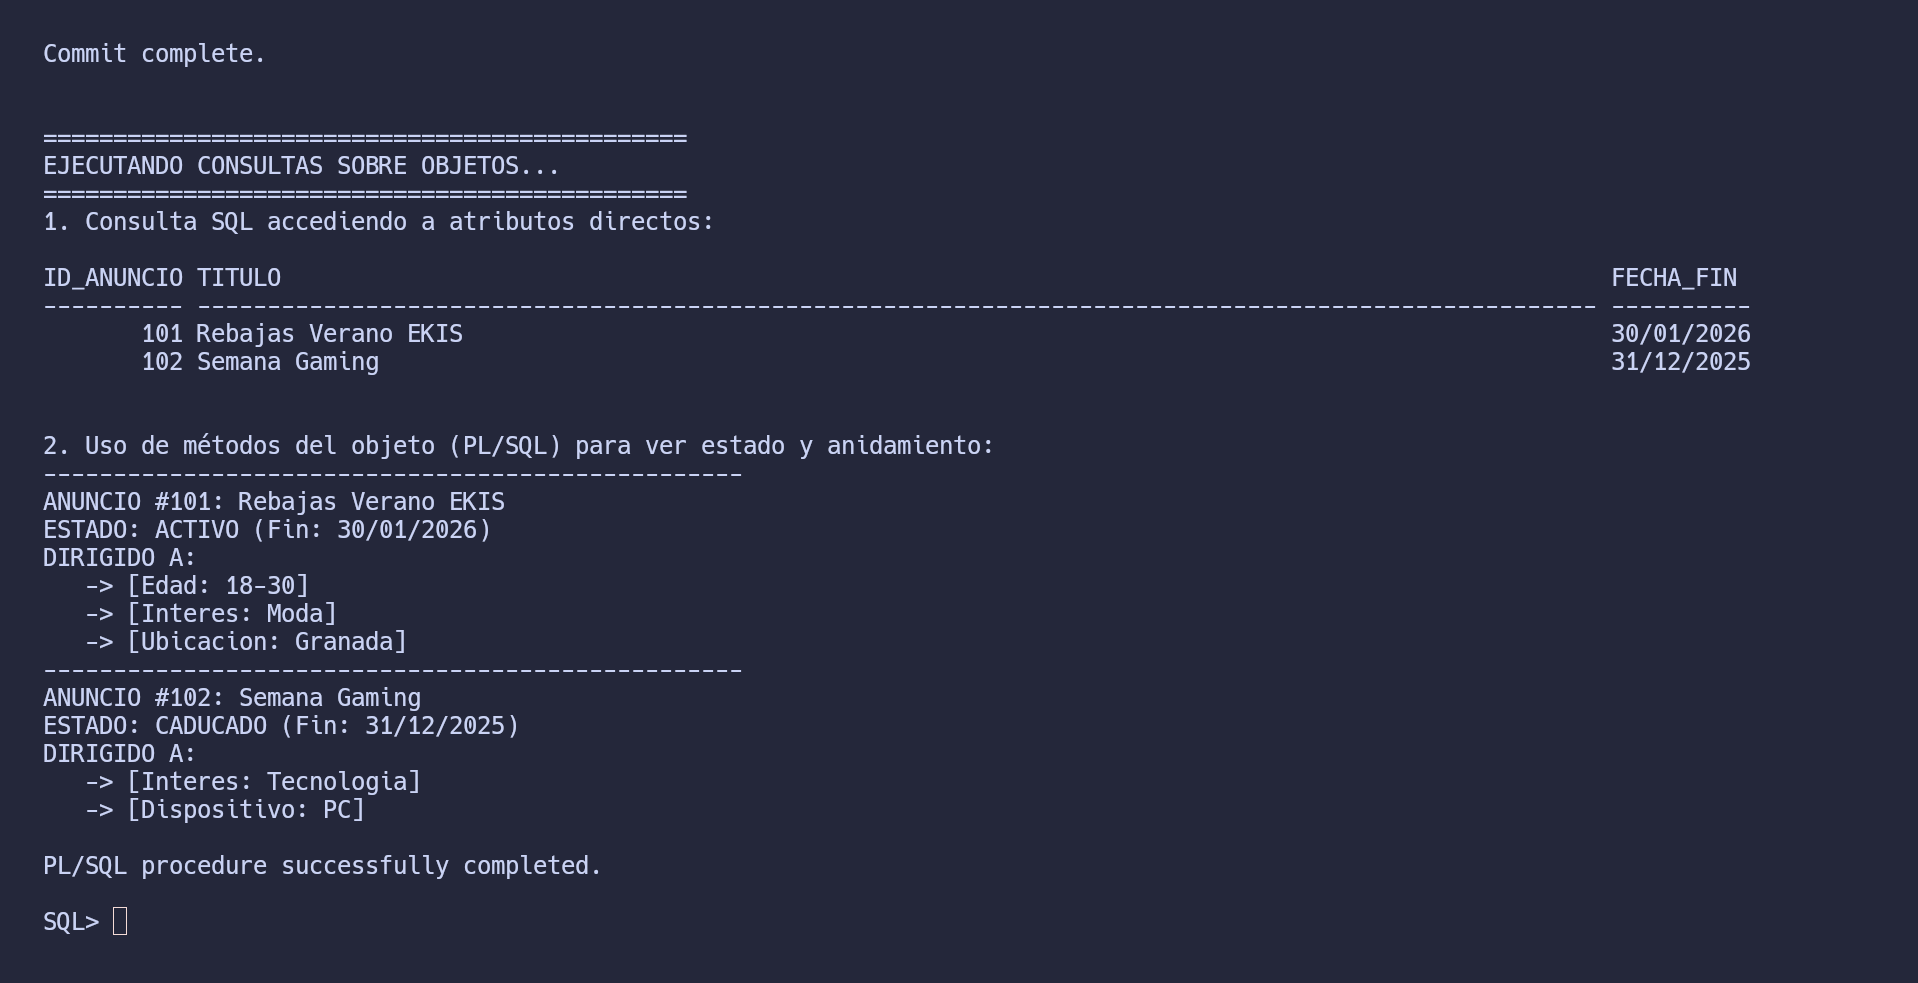
\includegraphics[width=0.9\textwidth]{figures/ismael/consulta_oracle.png}
    \caption{Ejecución de métodos sobre objetos Anuncio y recorrido de tablas anidadas en la terminal.}
    \label{fig:oracle_query}
\end{figure}

\section{Adecuación al Sistema EKIS}

El uso del modelo Objeto-Relacional para el módulo de Publicidad de EKIS presenta ventajas claras frente al relacional puro implementado en la práctica anterior:

\begin{itemize}
    \item \textbf{Encapsulamiento de Lógica:} La lógica para determinar si un anuncio es visible (\texttt{es\_activo}) reside en el propio objeto en la base de datos. Esto garantiza la consistencia, ya que cualquier aplicación que recupere el objeto obtendrá el estado correcto sin reimplementar la lógica de fechas.
    \item \textbf{Simplificación del Modelo:} El uso de \textit{Nested Tables} para el ''Público Objetivo'' elimina la complejidad de gestionar claves foráneas y tablas de unión manualmente para las características, permitiendo tratar el anuncio y sus criterios de segmentación como una unidad atómica lógica.
\end{itemize}
\newpage

% Escribe aquí tu parte. NO toques el main.
% Usa \section{}, \subsection{}, etc.
% Para imágenes usa: \includegraphics[width=\linewidth]{figures/TU_CARPETA/imagen.png}
\chapter{Modelo Documental (Javi)}

El modelo documental es una extensión del modelo clave-valor donde el valor es un documento estructurado (generalmente JSON, BSON o XML) que el sistema de base de datos puede entender, consultar e indexar. Para esta práctica, se ha elegido **MongoDB**, el gestor de base de datos NoSQL orientado a documentos más popular del mercado.

\section{Instalación y Configuración del Entorno}
Dado que el entorno de desarrollo se basa en sistemas Linux, se detalla el proceso de instalación tanto para distribuciones basadas en Arch Linux (sistema del alumno) como para Ubuntu/Debian (sistema de referencia).

\subsection{Instalación en Arch Linux}
En Arch Linux, los paquetes de MongoDB se encuentran gestionados a través del repositorio de usuarios (AUR), ya que la licencia cambió hace unas versiones.

\begin{enumerate}
    \item \textbf{Instalación del servidor:} Se utiliza un ayudante de AUR (como \texttt{yay}) para instalar los binarios:
    \begin{verbatim}
    yay -S mongodb-bin
    \end{verbatim}
    \item \textbf{Instalación de la GUI (opcional):} De igual forma, instalamos la interfaz gráfica oficial:
    \begin{verbatim}
    yay -S mongodb-compass
    \end{verbatim}
    \item \textbf{Inicio del servicio:} Habilitamos y arrancamos el demonio con systemd:
    \begin{verbatim}
    sudo systemctl enable --now mongodb
    \end{verbatim}
\end{enumerate}

\subsection{Instalación en Ubuntu/Debian}
Para sistemas basados en Debian, se puede cargar directamente usando el .deb.

\begin{enumerate}
    \item \textbf{Instalación de herramientas:}
    \begin{verbatim}
      sudo apt-get install gnupg curl
    \end{verbatim}
    \item \textbf{Importar la GPG key de MongoDB:}
    \begin{verbatim}
      curl -fsSL https://www.mongodb.org/static/pgp/server-7.0.asc | \
      sudo gpg -o /usr/share/keyrings/mongodb-server-7.0.gpg \
      --dearmor
    \end{verbatim}
    \item \textbf{Crear el archivo de lista correspondiente:}
    \begin{tabbing}
      echo "deb [ arch=amd64,arm64 \\signed-by=/usr/share/keyrings/mongodb-server-7.0.gpg ] \\https://repo.mongodb.org/apt/ubuntu jammy/mongodb-org/7.0 multiverse"\\ | sudo tee /etc/apt/sources.list.d/mongodb-org-7.0.list
    \end{tabbing}


    \item \textbf{Recargar base de datos y descargar mongodb:}
    \begin{verbatim}
      sudo apt-get update && sudo apt-get install -y mongodb-org
    \end{verbatim}
    \item \textbf{Descargar el .deb de la GUI (opcional):}
    \begin{verbatim}
      wget 
      https://downloads.mongodb.com/compass/mongodb-compass_1.46.10_amd64.deb
    \end{verbatim}
    \item \textbf{Instalar la GUI usando apt:}
    \begin{verbatim}
      sudo apt install ./mongodb-compass_1.46.10_amd64.deb
    \end{verbatim}
\end{enumerate}

\begin{figure}[h]
    \centering
    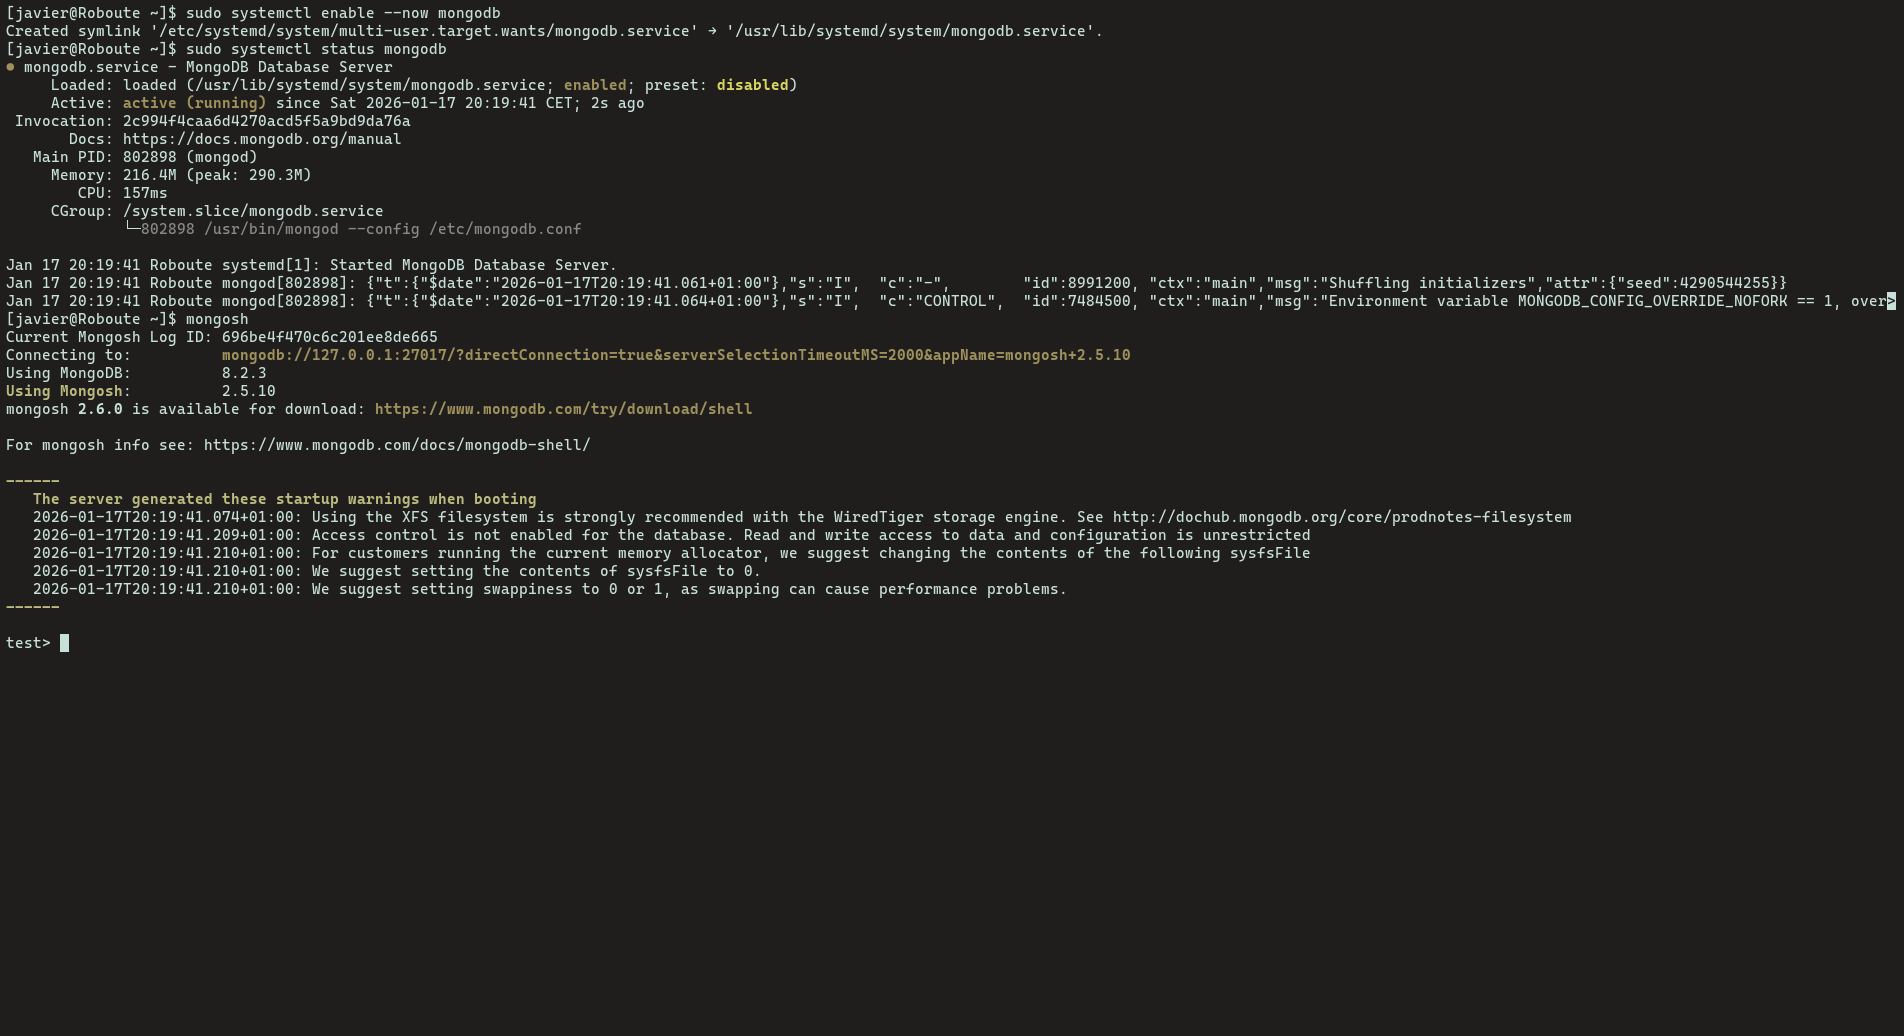
\includegraphics[width=\linewidth]{figures/javier/mongo_install_linux.png} 
    \caption{Shell de MongoDB ejecutándose en entorno Linux.}
    \label{fig:mongo_install}
\end{figure}

\section{Descripción del DDL y DML en MongoDB}
A diferencia de SQL, MongoDB no requiere una definición estricta de esquema (DDL explícito) antes de insertar datos. Las colecciones se crean automáticamente cuando se inserta el primer documento. No obstante, dispone de comandos equivalentes:

\begin{itemize}
    \item \textbf{DDL (Definición):}
    \begin{itemize}
        \item \texttt{use <db>}: Selecciona la base de datos (o la crea si no existe).
        \item \texttt{db.createCollection()}: Crea una colección explícitamente (opcional).
        \item \texttt{db.collection.drop()}: Elimina una colección (equivalente a \texttt{DROP TABLE}).
    \end{itemize}
    \item \textbf{DML (Manipulación):}
    \begin{itemize}
        \item \texttt{db.collection.insertOne()}: Equivalente a \texttt{INSERT}. Guarda documentos en formato BSON.
        \item \texttt{db.collection.find()}: Equivalente a \texttt{SELECT}. Permite filtrar por campos, incluso dentro de arrays o subdocumentos.
        \item \texttt{db.collection.updateOne()}: Equivalente a \texttt{UPDATE}. Utiliza operadores atómicos como \texttt{\$set} o \texttt{\$inc}.
        \item \texttt{db.collection.deleteOne()}: Equivalente a \texttt{DELETE}.
    \end{itemize}
\end{itemize}

\section{Implementación de Estructuras y Pruebas}
Para simular el subsistema de \textbf{Publicaciones} de EKIS en un modelo documental, aprovecharemos la capacidad de anidamiento. En lugar de tener tablas separadas para \texttt{PUBLICACION}, \texttt{HASHTAGS} y \texttt{COMENTARIOS} (como en el relacional), podemos tener una única colección \texttt{posts} donde cada documento contiene toda la información.

\subsection{Inserción de Datos (Creación)}
Creamos una publicación que incluye arrays para los hashtags y un subdocumento para la ubicación, demostrando la flexibilidad del esquema.
Las inserciones se pueden hacer desde la terminal o usando un .js en el que se definen las órdenes a ejecutar. De ahí se pasa a mongosh por entrada estándar.

\begin{lstlisting}[language=bash, caption={Inserción de una publicación con estructura compleja}]
use ekis_doc

db.publicaciones.insertOne({
  titulo: "Atardecer en la Alhambra",
  descripcion: "Disfrutando de las vistas con amigos.",
  usuario: "javier_ns",
  fecha: new Date(),
  likes: 0,
  tags: ["granada", "alhambra", "relax"],
  ubicacion: {
    ciudad: "Granada",
    lat: 37.176,
    lon: -3.588
  },
  comentarios: [] 
})
\end{lstlisting}

\begin{figure}[h]
    \centering
    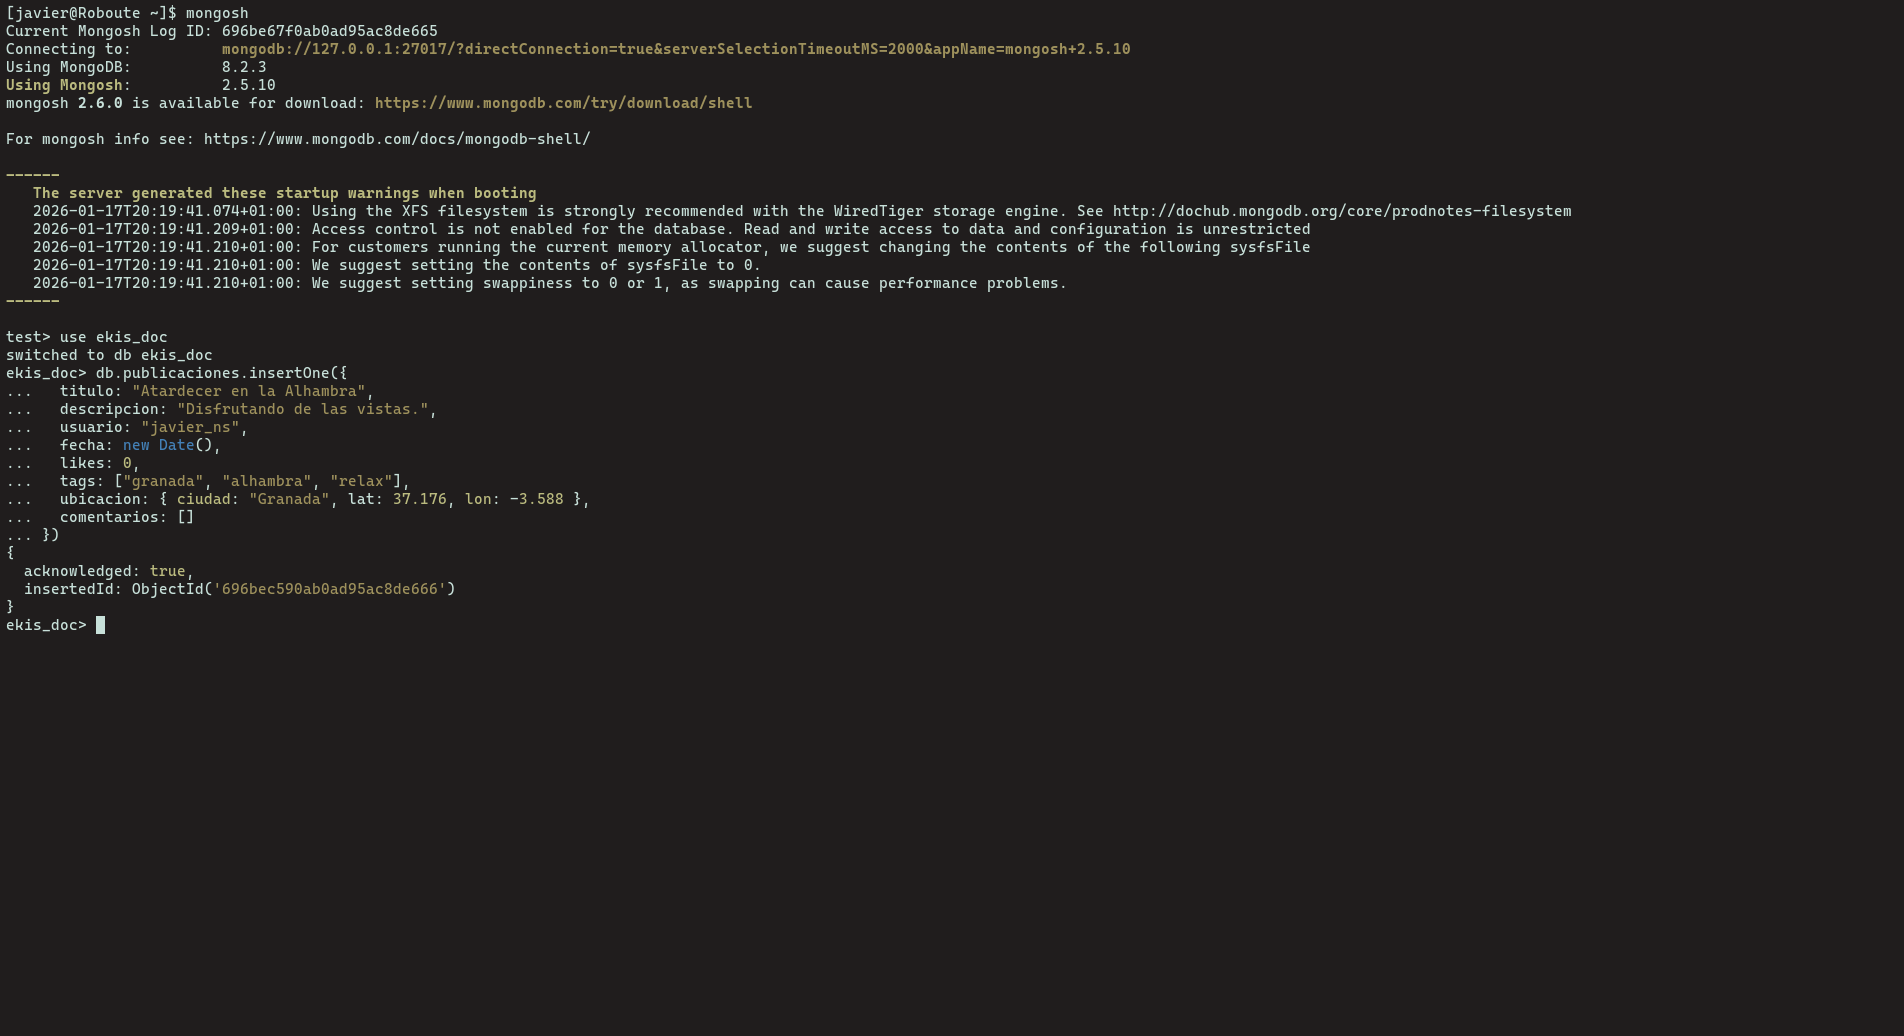
\includegraphics[width=\linewidth]{figures/javier/mongo_insert.png}
    \caption{Nueva publicación insertada en la colección \texttt{publicaciones}.}
    \label{fig:mongo_insert}
\end{figure}
\newpage
\subsection{Consultas (Lectura)}
Realizamos una consulta para buscar todas las publicaciones que contengan el tag "granada". Esto equivale a un \texttt{SELECT} con \texttt{JOIN} en SQL, pero aquí es una búsqueda directa sobre el array.

\begin{lstlisting}[language=bash, caption={Consulta por etiqueta (tag)}]
db.publicaciones.find({ tags: "granada" })
\end{lstlisting}

\begin{figure}[h]
    \centering
    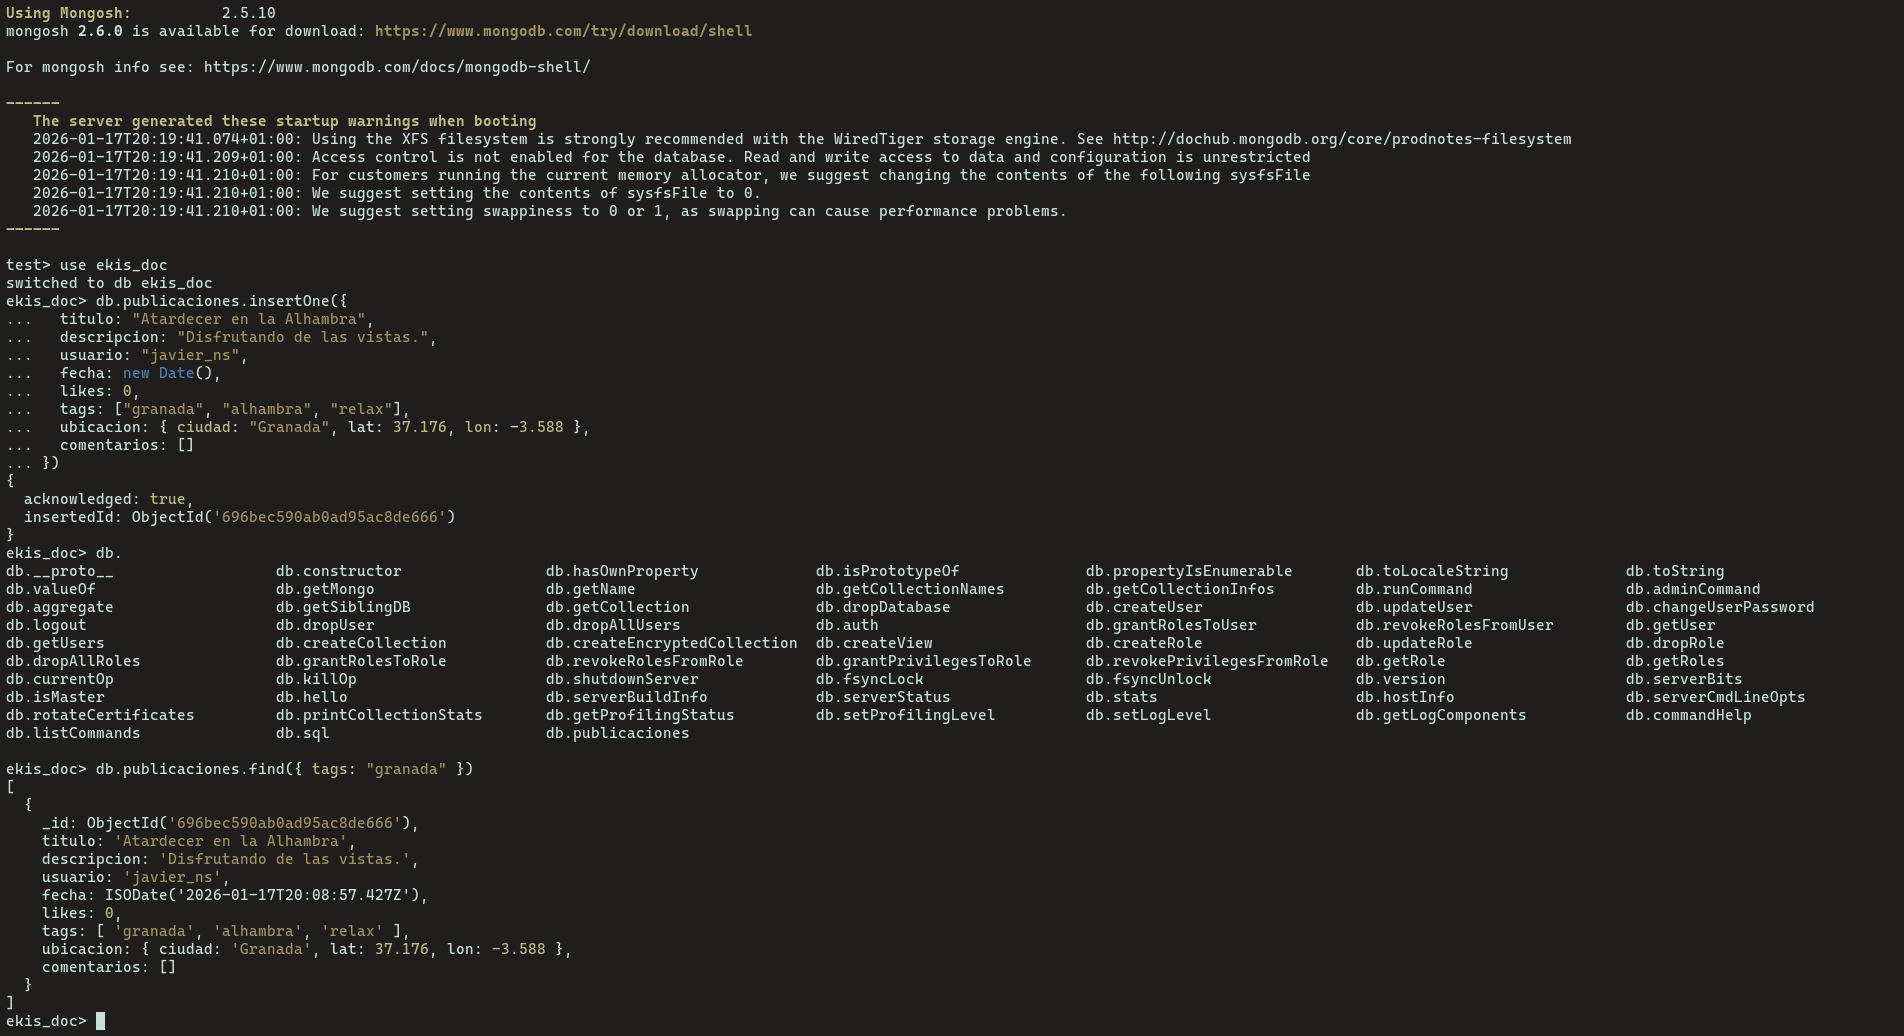
\includegraphics[width=\linewidth]{figures/javier/mongo_find.png}
    \caption{Resultado de la consulta filtrando por tags.}
    \label{fig:mongo_find}
\end{figure}
\newpage
\subsection{Modificación y Actualización}
Simulamos la acción de "Dar Like". En MongoDB podemos usar el operador \texttt{\$inc} para incrementar el contador atómicamente y \texttt{\$push} para añadir un comentario simultáneamente.

%TODO: Poner los acentos, ahora mismo se han quitado para que no den errores
\begin{lstlisting}[language=bash, caption={Actualizacion atomica: Like y Comentario}]
db.publicaciones.updateOne(
  { usuario: "javier_ns" },
  { 
    $inc: { likes: 1 },
    $push: { comentarios: { 
        usuario: "ismael_sm", 
        texto: "!Foton!",
        fecha: new Date() 
    }}
  }
)
\end{lstlisting}

\begin{figure}[h]
    \centering
    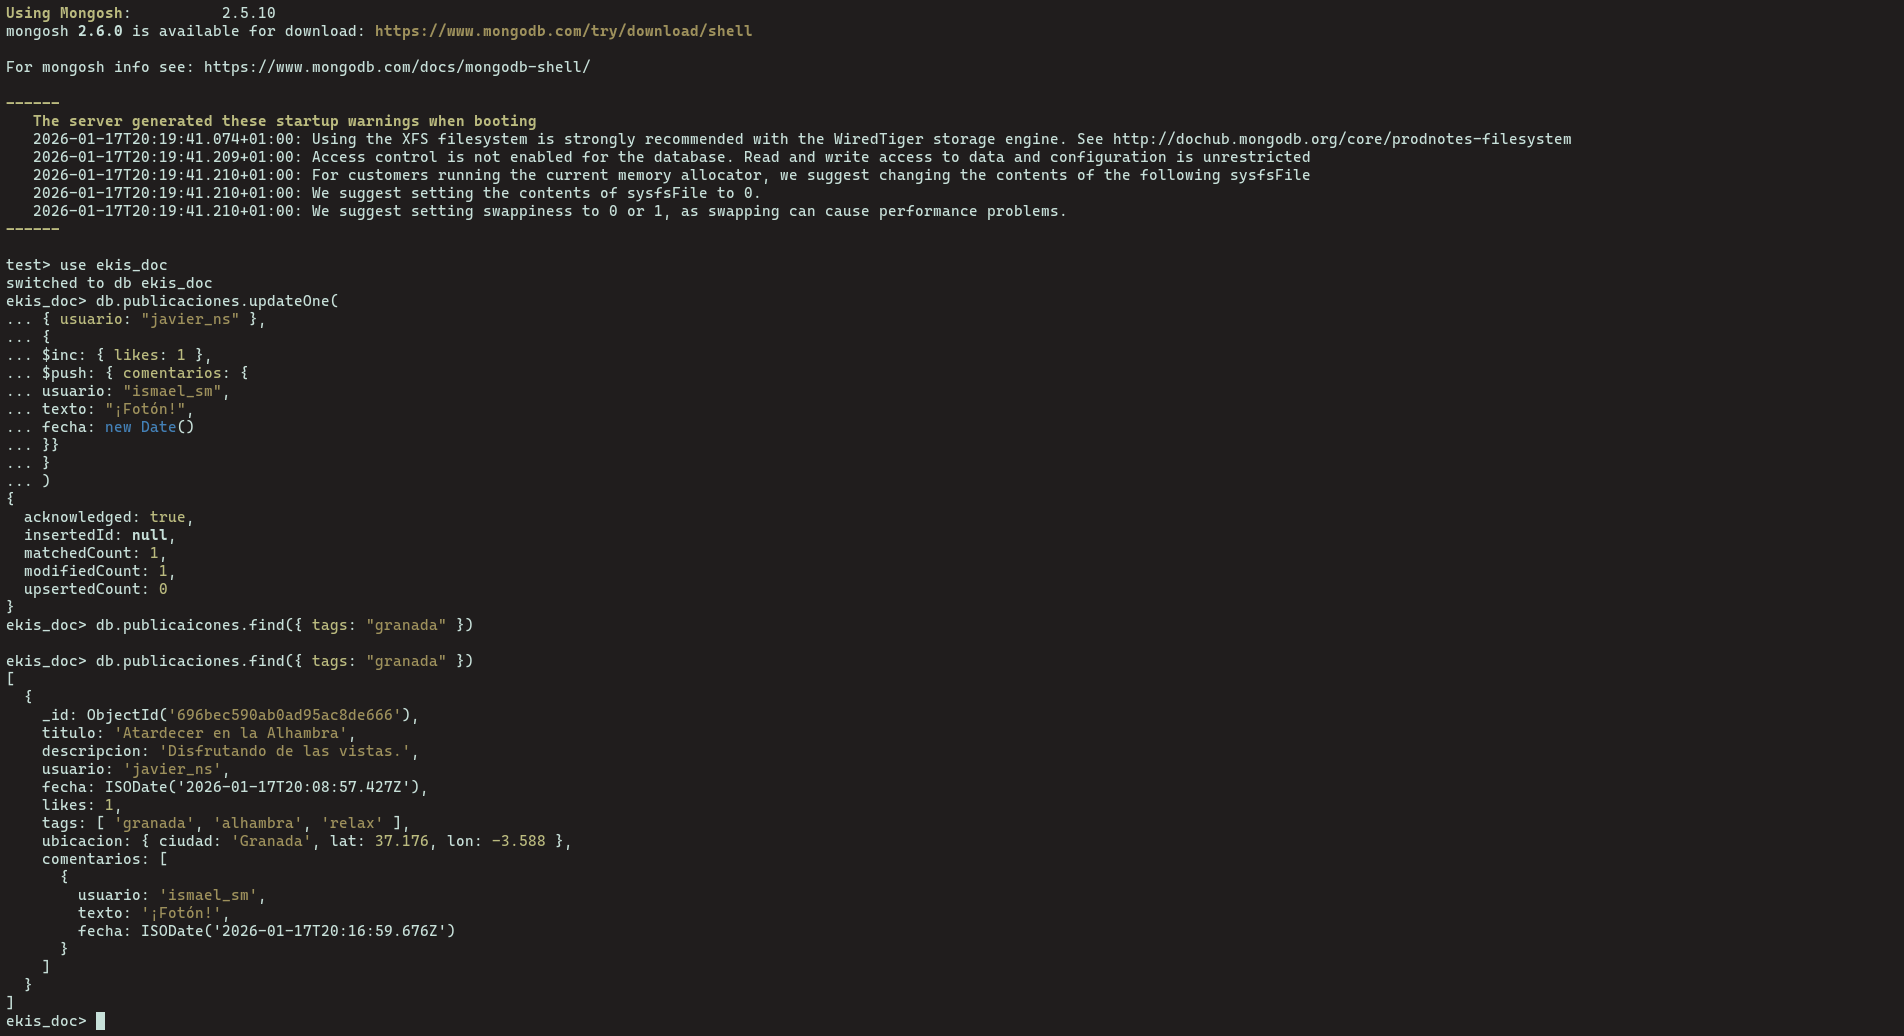
\includegraphics[width=\linewidth]{figures/javier/mongo_edit.png}
    \caption{Resultado edición de publicación.}
    \label{fig:mongo_edit}
\end{figure}
\newpage
\subsection{Borrado}
Finalmente, eliminamos la publicación creada.

\begin{lstlisting}[language=bash, caption={Eliminación del documento}]
db.publicaciones.deleteOne({ usuario: "javier_ns" })
\end{lstlisting}

\begin{figure}[h]
    \centering
    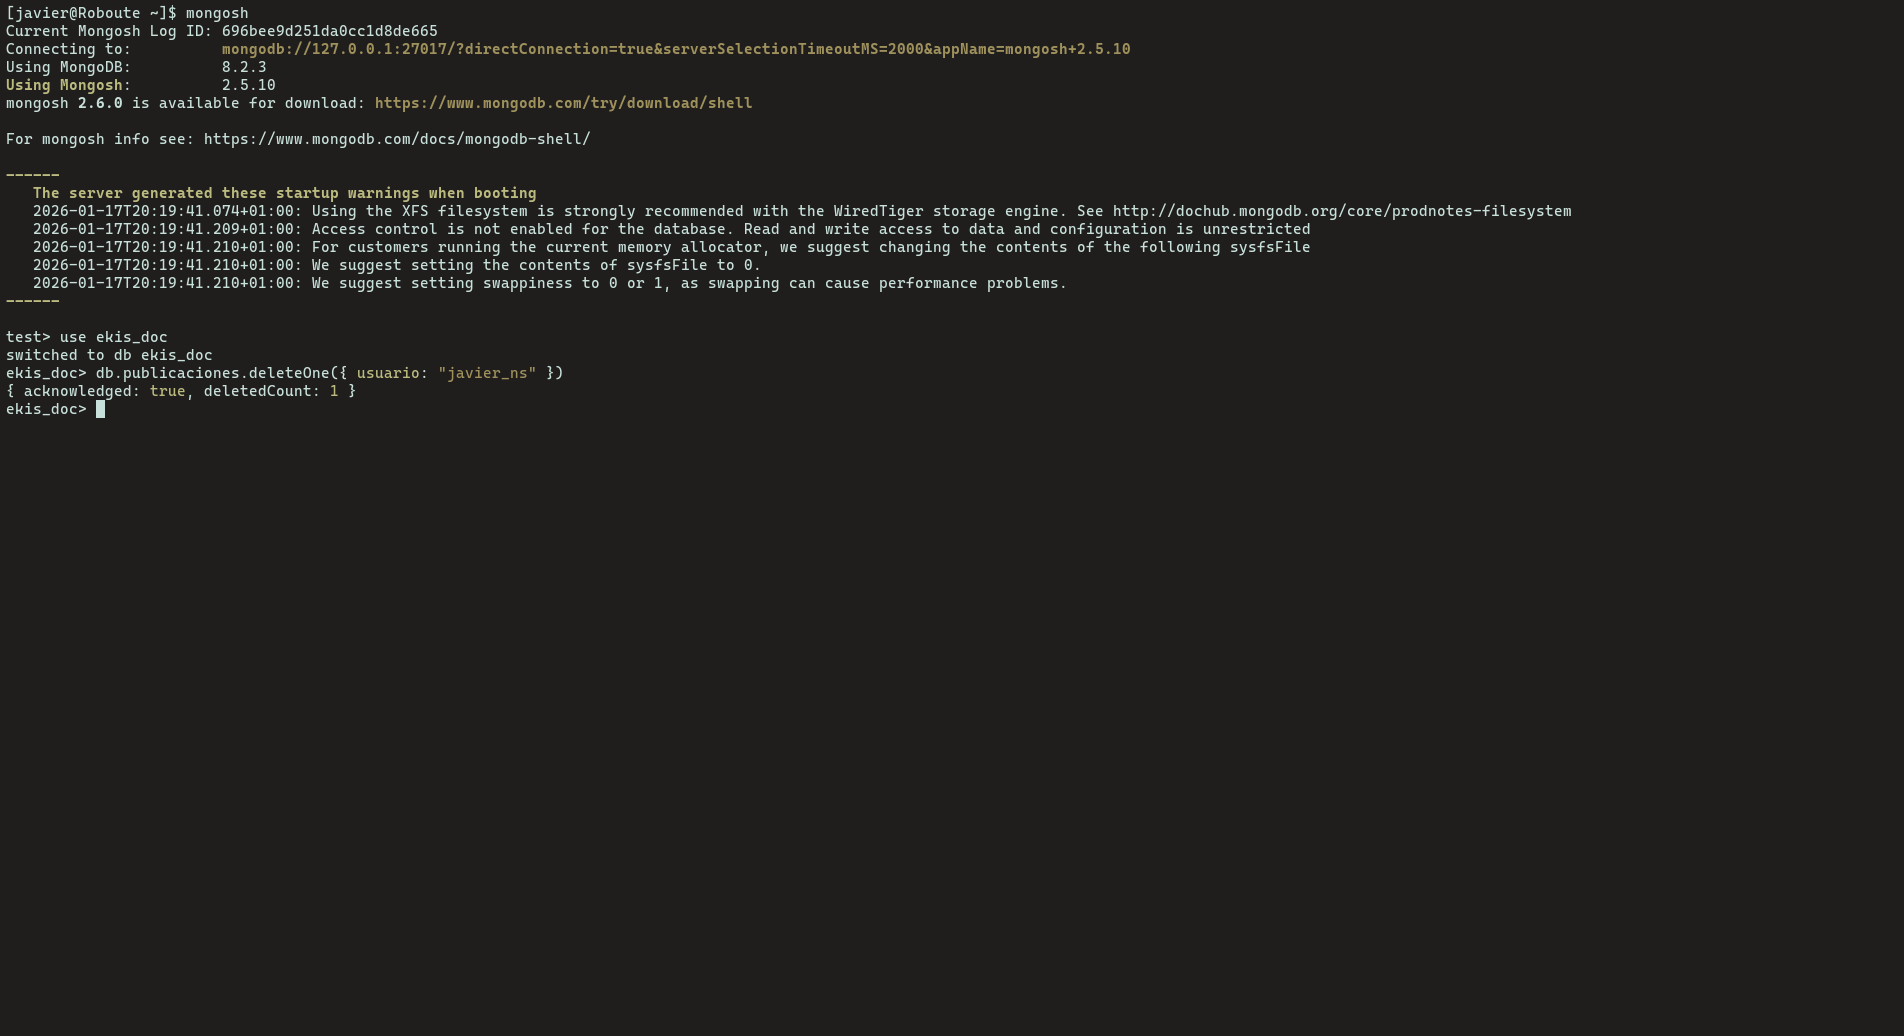
\includegraphics[width=\linewidth]{figures/javier/mongo_delete.png}
    \caption{Resultado de eliminación de publicación.}
    \label{fig:mongo_delete}
\end{figure}
\newpage
\section{Adecuación al Sistema EKIS}
El uso de un modelo documental con MongoDB presenta ventajas significativas para el subsistema de Publicaciones de una red social como EKIS:

\begin{itemize}
    \item \textbf{Flexibilidad de Esquema:} Las publicaciones pueden evolucionar. Algunos posts pueden tener encuestas, otros solo texto, y otros imágenes. SQL obliga a tener columnas nulas o muchas tablas; MongoDB permite que cada documento tenga campos distintos.
    \item \textbf{Rendimiento en Lectura (Feed):} Al guardar los comentarios y tags \textit{embebidos} dentro de la publicación, podemos recuperar toda la información necesaria para pintar el "Muro" con una sola lectura de disco, evitando los costosos \texttt{JOINS} del modelo relacional.
    \item \textbf{Escalabilidad:} Las redes sociales generan un volumen masivo de datos. MongoDB facilita el escalado horizontal (\textit{sharding}), distribuyendo las publicaciones en varios servidores de forma transparente.
\end{itemize}

Sin embargo, para datos altamente transaccionales y estructurados como la facturación de publicidad o la gestión estricta de usuarios, el modelo relacional sigue siendo superior por sus garantías ACID estrictas.

\newpage

% Escribe aquí tu parte. NO toques el main.
% Usa \section{}, \subsection{}, etc.
% Para imágenes usa: \includegraphics[width=\linewidth]{figures/TU_CARPETA/imagen.png}

\chapter{Modelo de Grafos (Jesús)}
\label{ch:jesus}

% Contenido de Jesús aquí...


\newpage

% Escribe aquí tu parte. NO toques el main.
% Usa \section{}, \subsection{}, etc.
% Para imágenes usa: \includegraphics[width=\linewidth]{figures/TU_CARPETA/imagen.png}

\chapter{Modelo Clave-Valor (Fer)}
\label{ch:fer}

El modelo \textbf{clave-valor} es una de las aproximaciones NoSQL más simples y eficientes: cada dato lo almacena como un par (\textit{key}, \textit{value}). A diferencia del modelo relacional, no existe un esquema rígido con tablas y columnas, sino un espacio de claves donde se consultan valores mediante accesos directos. Este enfoque resulta especialmente útil en sistemas con alta concurrencia, datos temporales y operaciones muy frecuentes, como los escenarios típicos de una red social.

Para este trabajo se ha seleccionado \textbf{Redis} como SGBD clave-valor de referencia, ya que combina velocidad (principalmente en memoria), facilidad de despliegue y un conjunto de estructuras de datos que permiten modelar relaciones y estados de forma sencilla.

\section{SGBD recomendado: Redis}

Redis (REmote DIctionary Server) es un sistema NoSQL clave-valor orientado a \textbf{rendimiento} y \textbf{baja latencia}, ampliamente utilizado como caché, gestor de sesiones, colas, contadores y almacenamiento temporal. Su valor añadido frente a un almacén clave-valor básico es que no solo almacena cadenas (\texttt{string}), sino también estructuras de datos de alto nivel como \texttt{hashes}, \texttt{sets}, \texttt{lists} o \texttt{sorted sets}, muy útiles para sistemas de interacción social.

\section{Instalación y Configuración del Entorno}

Redis es sencillo de desplegar en Linux y permite comenzar a trabajar en pocos minutos.

\subsection{Instalación en Ubuntu/Debian}
\begin{minted}{bash}
sudo apt update
sudo apt install redis-server
sudo systemctl enable --now redis-server
redis-cli ping
\end{minted}

Si todo es correcto, el comando \texttt{PING} responde con \texttt{PONG}.

\subsection{Instalación mediante Docker (alternativa)}
\begin{minted}{bash}
docker run -d --name redis-ekis -p 6379:6379 redis:latest
redis-cli -h 127.0.0.1 -p 6379 ping
\end{minted}

\section{Diseño Clave-Valor del Subsistema de Usuarios}

En una red social como EKIS, Redis se adapta especialmente bien a la gestión de:
\begin{itemize}
    \item \textbf{Sesiones y tokens} con caducidad (TTL).
    \item \textbf{Relaciones rápidas} (amistades, bloqueos) mediante conjuntos.
    \item \textbf{Contadores} (likes, seguidores) mediante incrementos atómicos.
    \item \textbf{Caché de perfiles} para acelerar lecturas frecuentes.
\end{itemize}

\subsection{Estrategia de claves}
Se define unas reglas simples para garantizar consistencia en el diseño:
\begin{itemize}
    \item \texttt{user:<id>} $\rightarrow$ datos del usuario en \texttt{HASH}
    \item \texttt{friends:<id>} $\rightarrow$ conjunto de amistades en \texttt{SET}
    \item \texttt{blocked:<id>} $\rightarrow$ conjunto de bloqueados en \texttt{SET}
    \item \texttt{session:<token>} $\rightarrow$ sesión activa en \texttt{STRING} con TTL
\end{itemize}

\section{Equivalencias DDL y DML en Redis}

\subsection{DDL (definición de estructura)}
Redis no requiere DDL tradicional (no existen \texttt{CREATE TABLE}). La estructura se define por el tipo de dato asociado a cada clave. En entornos reales, la consistencia del diseño se garantiza por convención de claves y por el código de la aplicación.

\subsection{DML (operaciones típicas)}
Redis se maneja con comandos directos:
\begin{itemize}
    \item \texttt{SET / GET} para valores simples (sesiones, flags).
    \item \texttt{HSET / HGETALL} para perfiles y datos agrupados en \texttt{HASH}.
    \item \texttt{SADD / SISMEMBER / SMEMBERS} para relaciones en \texttt{SET}.
    \item \texttt{INCR} para contadores atómicos.
    \item \texttt{EXPIRE / TTL} para caducidad (sesiones).
\end{itemize}

\section{Implementación y Pruebas}

A continuación se muestran operaciones reales que representan el subsistema de usuarios en EKIS usando \texttt{redis-cli}.

\subsection{Inserción de un usuario (HASH)}
\begin{minted}{bash}
HSET user:10 nombre "Fernando" email "fer@email.com" rol "user"
HSET user:20 nombre "Ismael"   email "isma@ugr.es"   rol "user"
HGETALL user:10
\end{minted}

\subsection{Creación de relación de amistad (SET)}
Para modelar amistad se usan conjuntos. Una amistad bidireccional se representa añadiendo cada usuario al conjunto del otro:

\begin{minted}{bash}
SADD friends:10 20
SADD friends:20 10
SMEMBERS friends:10
\end{minted}

\subsection{Control de coherencia: evitar auto-relación}
Redis no tiene \textit{triggers}. La regla “no puedo ser amigo de mí mismo” se controla desde la lógica de aplicación (o mediante scripts Lua). Por ejemplo, la aplicación tiene que impedir:
\begin{minted}{bash}
SADD friends:10 10
\end{minted}

\subsection{Bloqueo de usuario (SET) con consistencia}
Cuando un usuario bloquea a otro, es coherente eliminar la amistad previa y registrar el bloqueo. Redis nos permite agrupar operaciones con \texttt{MULTI/EXEC}:

\begin{minted}{bash}
MULTI
SREM friends:10 20
SREM friends:20 10
SADD blocked:10 20
EXEC
\end{minted}

\subsection{Gestión de sesión con caducidad (TTL)}
Las sesiones son un caso ideal para Redis porque permite caducidad automática:

\begin{minted}{bash}
SET session:token_abc "10"
EXPIRE session:token_abc 3600
TTL session:token_abc
GET session:token_abc
\end{minted}

\subsection{Ejemplo práctico con Python (redis-py)}
Redis se integra fácilmente con Python para automatizar pruebas y lógica de negocio:

\begin{minted}{python}
import redis

r = redis.Redis(host="127.0.0.1", port=6379, decode_responses=True)

# Crear usuario (HASH)
r.hset("user:10", mapping={"nombre": "Fernando", "email": "fer@email.com", "rol": "user"})

# Añadir amistad (SET)
r.sadd("friends:10", "20")
r.sadd("friends:20", "10")

# Crear sesión con TTL
r.set("session:token_abc", "10")
r.expire("session:token_abc", 3600)

print("Usuario 10:", r.hgetall("user:10"))
print("Amigos de 10:", r.smembers("friends:10"))
print("TTL sesión:", r.ttl("session:token_abc"))
\end{minted}

\section{Adecuación al Sistema EKIS}

El modelo clave-valor con Redis es especialmente adecuado en EKIS como soporte de alto rendimiento para el subsistema de usuarios:

\begin{itemize}
    \item \textbf{Baja latencia y alta concurrencia:} ideal para operaciones muy frecuentes como consultas de estado, contadores y relaciones.
    \item \textbf{Sesiones y expiración automática:} permite gestionar tokens de autenticación y sesiones sin necesidad de procesos de limpieza.
    \item \textbf{Relaciones rápidas con SET:} amistades, bloqueos y listas de seguimiento se resuelven con operaciones eficientes.
    \item \textbf{Soporte natural para caché:} reduce carga en el SGBD relacional principal cuando se consultan perfiles repetidamente.
\end{itemize}
sin embargo, Redis no sustituye completamente al modelo relacional cuando se requieren consultas complejas, \texttt{JOIN}, o garantías transaccionales fuertes a nivel de múltiples entidades.

\newpage

% Escribe aquí tu parte. NO toques el main.
% Usa \section{}, \subsection{}, etc.
% Para imágenes usa: \includegraphics[width=\linewidth]{figures/TU_CARPETA/imagen.png}

\chapter{Modelo Columnar (Sergio)}
\label{ch:sergio}

% Contenido de Sergio aquí...


\newpage


% ----------------------- %
% BIBLIOGRAFÍA
% ----------------------- %

% Estilo de cita.
\bibliographystyle{apa-good}
%\renewcommand\bibname{Reference}

%[citestyle=numeric]

%\renewcommand\bibname{Bibliografía}
%

% Añadimos la bibliografía al índice
\phantomsection
\end{document}
